\documentclass[UTF8]{ctexart}
\usepackage[T1]{fontenc}
\usepackage[UTF8,heading = true]{ctex}

% Language setting
% Replace `english' with e.g. `spanish' to change the document language
% \usepackage[english]{babel}
\usepackage{color}

% Set page size and margins
% Replace `letterpaper' with `a4paper' for UK/EU standard size
\usepackage[letterpaper,top=2cm,bottom=2cm,left=3cm,right=3cm,marginparwidth=1.75cm]{geometry}

% Useful packages
\usepackage{amsmath}
\usepackage{graphicx}
\usepackage{braket}
\usepackage{array}
\usepackage{longtable}
% Adding 
\usepackage[colorlinks=true, allcolors=blue]{hyperref}

\title{多立恒网页使用指南}
\author{司迎}
% \date{2024年12月6日}
\begin{document}
\maketitle
\tableofcontents
\begin{abstract}
非官方文件,仅以新郑公司的实际使用情况为参考。因为是自编自用的使用补充说明,也不是写论文,所以文本编辑风格比较口语化,建议不要从这一篇文档开始熟悉系统。仅需点开网址页面即可查看的讲解部分不做截图展示。官方文件是《河南中原燃气有限公司瓶装燃气平台项目-功能说明文档》,可自行查看。

这个文档包含多立恒3.0网页使用时的各种功能的补充说明,以及各模块互相关联的总结,需要注意的事项。因为时间问题未完成,有些更新的部分未补充,需要后台管理员持续更新。功能说明是指只要点开网页的每个模块、每个可选的选项卡都查看一遍,即可一目了然的事实情况的归纳,没有什么含金量,看不明白可以自己在网页上点一点自己思考一下对应内容是什么含义;各模块相互关联的总结是指各模块的嵌套关系与关联影响,大部分根据经验总结,受业务范围和软件更新限制,不一定全面也不一定一成不变;需要注意的事项指的是一些即使点开网页或app即可一目了然,但仍然会因为业务信息不同步或粗心大意造成误解或误选的内容。这三类内容在文档中没有明显标识,注意事项和一些奇怪的功能一般会用红字突出显示。

使用该指南时可点击对应索引查看,或使用ctrl+F直接在页面内关键字搜索。在按顺序使用系统之前,建议先从“设置--场站配置--流程配置”中了解气瓶正常流转的完整顺序。但是这一部分该文档没有来得及写,所以需要自行在系统后台查看了解。
\end{abstract}

\section{首页}

首页左上角展示默认仪表盘,展示内容根据角色权限可以自行调整,管理员默认可以查看所有信息,但也可以在角色权限内调整。

除了角色权限内所显示的版块外,默认仪表盘处点开也可“新建仪表盘”,自定义使用页面首页需要展示的内容,并且可随时展示各种版本页面。首页仪表盘编辑见Figure \ref{fig:preface1}

首页右上角的“通知公告”可以点开查看网页有哪些最近的更新,有些功能需求的上线通知会列在里面。
\begin{figure}[h]
	\centering
	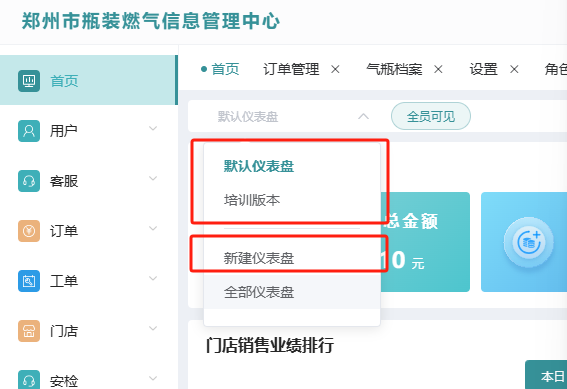
\includegraphics[width=0.7\linewidth]{D:/latex/dlh_tutorial_figs/preface1}
	\caption{首页仪表盘}
	\label{fig:preface1}
\end{figure}

\textcolor{red}{多立恒网页多个可查询的页面(押金管理、退瓶管理、欠瓶管理、合同管理、保单管理、订单管理、订单售后、充装记录、气瓶档案)都能自定义设置显示列,也可以设置查询框中的默认查询条件。}详情见多立恒首页2024/04/09系统升级公告。如果需要新增查询条件或新增显示字段,可以先从“设置列”和“设置查询条件”的入口查看是否可以直接添加。“安检单管理”模块中没有“设置查询条件”功能。

注意:有些页面的时间类查询条件,系统有默认当天的值,并且不展开查询框就无法直接看到那个查询条件。因此,如果你未设置过查询条件,可能会在不知情的情况下找不到你要查询的内容。出现这类情况可先展开所有的查询条件,排查是否有已写入的值,删掉查询条件内容或者选择你所需的查询条件,再次点击查询即可显示有效信息。

\section{用户}

见《河南中原燃气有限公司瓶装燃气平台项目-功能说明文档》4.3。

\subsection{用户管理}
从用户管理中可以查看所有已开户的用户信息,可根据上方的查询条件查询,并导出正式用户表格。用户管理可以通过户号查询,需要手动在设置查询条件内添加。每个用户信息条目右侧可以进行编辑等操作。

用户户号等蓝色标识的内容均可点击进入详细页面,其中比较常用的是“户号”中的内容,可在其中查看用户信息,全部的押金信息,合同信息,订单信息,在用气瓶,以及安检记录等。

\subsection{保单管理}
公司无保险业务,未使用此功能。

\subsection{押金管理}
新郑公司财务不使用此功能,一般信息部作为核查使用。这个功能不好用的点在于拍照内容需要人工审核,押金单内容与拍照的纸质押金单内容不一定一致,有参考价值,但如果作为实际押金收据的证明则因存在监管漏洞而不适用。

包含“正常单据”,“已作废”两个页面,可填充查询条件筛选押金数据。

押金管理可新增押金单,携瓶入户,批量作废,批量回执,导出。列表中,蓝色字体的押金单号和户号可以点开查看详细信息。

每条押金单信息可新增,编辑,作废,退瓶,回执,打印。押金单的编辑功能可编辑所属机构、气瓶类型、数量、押金单价、租金、起租日期、支付方式、经办人、修改或删除、新增押金单照片。用户信息和随单生成的押金单号不能修改。

退瓶功能关联配送员好运气app中的退瓶功能,确认退瓶后会生成一个退瓶单号,对应配送员的手机app中会接到退瓶单并且上门扫码退瓶。押金退款只能走现金途径,无法直接从微信中退回。已退气瓶的退瓶单会更新在“退瓶管理”模块中。

\subsection{退瓶管理}

退瓶后的信息在退瓶管理中更新,可通过退瓶单号、押金单号等相关项查询,退瓶需在网页端手动点确认。

\subsection{欠瓶管理}

一般情况下不允许欠瓶,在随单的“新增欠瓶”功能可自主配置之前,会有配送员在实际操作中本应“新增押金”而错选成了欠瓶,这类情况需要库房营业员将这些欠瓶单全部作废,并按相应的用户和商品规格数量新增押金单,保证数据正常。

\subsection{合同管理}

每个用户都需要跟公司签署供气协议,供气协议上传在合同模板,配置在随单任务中。未签署合同的用户在他的新订单完成前,会与随单安检一起列在随单任务中;已签署合同的用户则不需要再签,签合同入口也不会在随单任务中出现。点开合同编号可查看合同详情。

在某次系统更新后,新郑公司的所有“瓶批”、“槽批”类型的用户,签署合同时都会出现“合同模板获取失败”的提示,从而无法签署合同。目前的处理方式是每次遇到该问题,都由配送员在app端按实际用气情况手动为用户修改用户类型为“居民”、“商业”或“工业”。

\textcolor{red}{注意}:
合同管理需要经常(一般是每天)筛选“待我方签署”的合同,批量选择完成签署,用户的合同才会被盖上电子公章。同时,有些早期积压的“待客户签署”的合同,也需要定期找到并撤销,以免后续配送员为这个用户新签合同时导致“用户已发起过相同模板”的提示。



\section{客服}

见《河南中原燃气有限公司瓶装燃气平台项目-功能说明文档》4.2。

\subsection{通话分析}

见《河南中原燃气有限公司瓶装燃气平台项目-功能说明文档》4.2.5。


\subsection{通话记录}

见《河南中原燃气有限公司瓶装燃气平台项目-功能说明文档》4.2.4。

\section{订单}

订单是与配送工作关联最大的模块。客服、营业员、运维人员最主要关注的就是这个模块。
\begin{itemize}
	\item \textbf{订单管理}一个订单生成后,会分别进入待指派--配送中--待签单--已签收的流程,若订单生成后未完成,微信未支付取消,或代客下单取消的订单,会生成在“已关闭”选项卡中。
将订单的各个流程状态分别展示在不同的选项卡中以供查询;
    \item \textbf{订单售后}是已支付的订单,在订单完成前从用户端申请退单的订单信息。
\end{itemize}
\subsection{订单管理}

订单管理的字段包含几乎所有订单、用户、气瓶流转信息。

Tips: 有订单管理权限即可看到气瓶全流程追溯,点开订单号,下拉页面的商品扫码数、包装物扫码数,不为0的情况下都可以点开数字查看编号详情,蓝色字体的编号可点开查看气瓶、充装、流转的全部信息;或直接在页面的“商品芯片编码”等列直接查看编码,可点开查看详细流转信息。若需查询气瓶编号,可将相应筛选条件下的订单导出,在表格中筛选再回到订单中查看;或在相应筛选条件的页面内通过ctrl+F直接搜索。

订单管理包含多个选项卡,每个选项卡的字段都略有不同,注意导出数据时的选择。以下是订单管理页面的字段及释义。

\begin{longtable}[h!]{ | m{3cm} | m{12cm} | } 

		\hline
		订单号 & 订单生成的唯一编号,D+日期+订单序号,页面内可点开查看详细信息,详细右侧的订单日志可查看订单流转状态。\\
		\hline
		商品 & 格式为: 商品\^{}规格\^{}价格\^{}数量;不同规格的商品用逗号隔开\\
		\hline
		数量 & 商品列中所有规格商品的数量总和\\
		\hline
		门店 & 用户的就近门店,用户管理中保存的就近门店会根据订单的派单、配送人员的所在库房更新\\
		\hline
		户号 & 开户后生成的唯一户号,并对应唯一用户二维码,用户相关所有信息(基础信息,订单,安检等)与此户号关联。\\
		\hline
		催单次数 & (新系统已经没有这一项了)系统催单次数,一般是客服权限\\
		\hline
		用户名称& 用户开户时的自定义名称\\
		\hline
		用户类型& 用户类型,可在用户管理中编辑\\
		\hline
		用户标签& 给用户添加的标签,未使用\\
		\hline
		联系人& 用户下单时填的联系人,一般与用户名称一致\\
		\hline
		联系电话& 用户开户电话。在“待指派”、“配送中”、“已签收”三个选项卡中,这个字段名称是“电话号码”\\
		\hline
		省& 用户地址所在省\\
		\hline
		市& 用户地址所在市\\
		\hline
		区& 用户地址所在区\\
		\hline
		街道& 用户地址所在街道\\
		\hline
		地址& 用户开户地址,用户端无法编辑,app和网页端可编辑,一般由配送工或客服编辑修改。 \\
		\hline
		业务员& 如果是配送员为用户开户,则会填充业务员,对应配送员的名称。\\
		\hline
		会员卡号& 与户号一样,一户一会员号。如果有优惠服务可在此处使用查看。\\
		\hline
		欠瓶单& 关联该订单的欠瓶单。送出瓶数大于回收瓶数,且未开押金单时新增欠瓶单。\\
		\hline
		关联押金单& 押金单,页面中可点开查看详情。\\
		\hline
		预约时间& 用户微信下单时的预约时间,立即配送,或一个可选时间段\\
		\hline
		自提& 现在这个系统只有配送,没有自提完成订单的关联操作,所有都是否。\\
		\hline
		购买方式& 不知道除了购买还有什么其他方式。 \\
		\hline
		支付方式& 用户实际支付方式,目前微信下单必须是微信支付,代客下单只能现金支付。\\
		\hline
		支付状态& 订单当前支付状态,会根据订单流程动态更新\\
		\hline
		订单状态& 订单当前状态,会根据流程动态更新\\
		\hline
		售后状态& (如有)退单、退货办理进度\\
		\hline
		开票状态& 关联的电子发票功能,未使用\\
		\hline
		商品金额& 商品规格数量的金额总计 \\
		\hline
		商品积分& \\
		\hline
		运费& 在设置--配送设置--运费设置中的运费规则,根据用户地址楼层\\
		\hline
		订单应收& 数值与商品金额一致,前面多了货币符号\\
		\hline
		订单实收& 实际收取金额,前面有货币符号\\
		\hline
		退残重量& 目前这个系统没有退残的关联操作\\
		\hline
		退残金额& 目前这个系统没有退残计价的关联操作\\
		\hline
		押金金额& 如果该订单有关联押金单,押瓶类型和数量对应的总金额\\
		\hline
		结算金额& 商品金额+押金金额\\
		\hline
		下单人& 微信下单时就是用户名,代客下单时就是配送员名称\\
		\hline
		下单时间& 订单生成时间\\
		\hline
		来源& 微信、代客下单、客服坐席等下单方式\\
		\hline
		派单方式& 一般都是指定人员,没试过自动派单,不知道会显示什么。\\
		\hline
		处理人& 配送员名称\\
		\hline
		配送状态& 订单当前配送状态\\
		\hline
		签收人& 不知道为什么都是配送员的名字\\
		\hline
		签收时间& 订单完成时间,精确到秒\\
		\hline
		商品扫码数& 送出重瓶的扫码数量\\
		\hline
		包装物扫码数& 收回空瓶的扫码数量\\
		\hline
		押/欠瓶数& 押x欠x,随单新增押金或新增欠瓶的数量\\
		\hline
		商品气瓶编号& 扫码送出重瓶的气瓶镂空码\\
		\hline
		商品芯片编码& 扫码送出重瓶的芯片编码\\
		\hline
		包装物气瓶编号& 扫码收回空瓶的气瓶镂空码\\
		\hline
		包装物芯片编码& 扫码收回空瓶的芯片编码\\
		\hline
		签收偏差(km)& 小写km,中文全角括号。用户填写地址与配送时的手机定位的偏差距离\\
		\hline
		配送耗时(分钟)& 中文全角括号。订单生成至订单完成的时间差\\
		\hline
		回执状态& (新系统已经没这一项了)需手动回执,目前财务计划用来核销订单。需要注意,点了“回执”的订单,将会从“已签收”中去除,显示在“已回执”中。因此,如需导出某时间段内已签收的订单,最好从“全部”中,根据签收时间筛选导出,不然就需要在“已签收”“已回执”两个选项卡页面分别导出。\\
		\hline
		回执人	& 仅为公司财务、库房营业员开启回执人权限 \\
		\hline
		回执时间& 点击回执的时间,(后续若有撤销回执的操作,则下次回执时间将覆盖上次已撤销的回执。)这个功能已经聊过了,应该是不会有了。\\
		\hline
		付款时间& 新郑公司财务需求,新增的付款时间\\
		\hline
		备注& 订单备注,如代客下单商品规格选错等情况。\\
		\hline
		\textcolor{red}{关于气瓶编号芯片编码}& \textcolor{red}{取决于扫码时所选择的类型:芯片编码、气瓶编号、气瓶码。在配送阶段未验证建档的情况下,如果在app里选择气瓶码扫了芯片码,那么芯片码会存储在气瓶码一列,且该扫码不会被记录在溯源流程中。}\\
		\hline

\end{longtable}


\subsection{订单售后}

发起退款(退单、退货)订单会在订单售后中显示,分为“待审核”、“已审核”、“已完成”、“已关闭”四种状态。订单售后流程见Figure \ref{fig:chargeback}.

\begin{figure}[h]
	\centering
	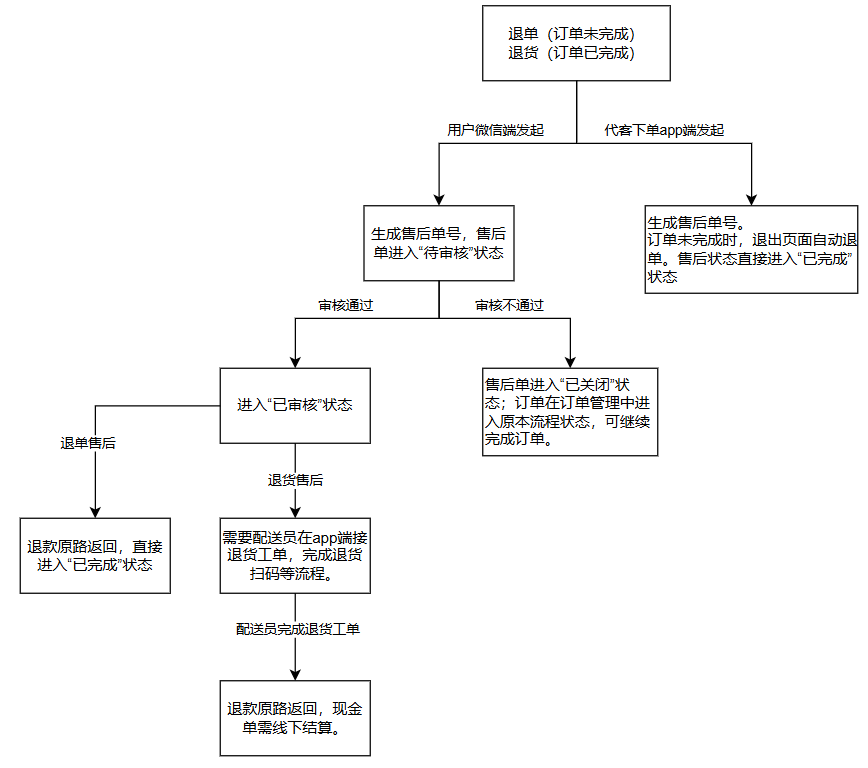
\includegraphics[width=1\linewidth]{dlh_tutorial_figs/chargeback}
	\caption{订单售后流程}
	\label{fig:chargeback}
\end{figure}


\subsection{回收}

从运气到家app端,首页-工单-回收,进入回收页面,若权限开放可新增回收项目。若只开放转派权限,则由客服接听电话时在网页端新增回收工单,派给配送员,从手机端接“回收”工单,配送员无法自主新增。

这一部分用法有限,并且难以监管,可根据公司实际运营要求使用。一般此类工单可走线下的现金和纸质单进行处理,线上单据对于无智能手机的用户来说非常不便。

\begin{itemize}
	
	\item 残液回收,公司不回收残液。气瓶残留的液化气到气站要抽残处理不做二次利用。
	
	\item 气瓶回收,可以根据公司要求的气瓶规格、年限定价,新增回收单。
	
	\item 商品置换,不知道置换什么。
	
\end{itemize}


\subsection{交易流水}

可以根据单据类型查询,有“订单收款”、“押金收款”、“会员充值”、“会员还款”。
可以根据交易流水号或交易单据号,在微信支付平台查询交易信息和付款人电话,根据电话可在订单管理或用户管理中查到对应订单和用户。20250419已切换银盛支付,不能在微信支付平台中查询相关交易信息了,需要结合民生银行、银盛支付后台查看。


\section{工单}

\subsection{工单管理}

工单管理的分类可在“设置-工单配置-工单配置”中新增并启用。

\subsection{附加工单}




\section{门店}

\subsection{门店管理}

门店管理可以自定义门店区域范围,门店营业时间,地址等信息。这里设置的门店营业时间将会在微信公众号对应门店的用户手机端显示。用户开户时填写的地址,会根据此处定义的区域范围给用户赋予一个就近门店。用户门店会在用户实际下单被派单配送时根据配送员所属门店更新。


门店区域范围可以自定义选点划线设置。



\section{安检}

\subsection{安检单管理}

\subsection{隐患记录}


\section{配送}


\section{气站}

整体内容详情可见《河南中原燃气有限公司瓶装燃气平台项目-功能说明文档》4.1.1至4.1.11

\subsection{气瓶档案}

见《河南中原燃气有限公司瓶装燃气平台项目-功能说明文档》4.1.2至4.1.5,以及4.1.8、4.1.9。

\subsection{充装记录}

见《河南中原燃气有限公司瓶装燃气平台项目-功能说明文档》4.1.6。

\subsection{气站管理}



\subsection{气瓶分析}

见《河南中原燃气有限公司瓶装燃气平台项目-功能说明文档》4.1.11。

\begin{enumerate}
	\item 气瓶分析
	
	\begin{itemize}
		
		\item 选择站点。
		
		\item 气瓶投放分析。可以选择年份查看当年每个月气瓶建档的数量。
		
		\item 充装分析。可按月查看当月每天的充装瓶数,也可按年查看当年每月的充装瓶数。
		
		\item 充装回流率。气瓶建档3-6个月内回站充装的比例。
		
	\end{itemize}

	\item 沉睡气瓶分析
	所有查询项都可自行点开查看是否符合某次数据的导出需要,这里介绍几个主要用到的查询项,还有看起来容易造成迷惑的“关联单据号”项:
	\begin{itemize}
		
		\item 流转节点。一个气瓶的全流程追溯节点有列出。除了“通用流程”中的正常流转节点以外,还保存有送检、报废、商品回收置换(这部分新郑公司未使用)、欠瓶、退货、安检扫瓶等等非流转性质的扫码流程。但是亲测以上提到的“安检扫瓶”、“气瓶报废”等流程什么都查询不出来,所以这里只是列出来,但多立恒未实际将这些节点纳入可追溯的条件。
				
		\item 最后机构。最后位置的责任人或站点所在的机构,对应门店--门店管理--门店名称,以及气站--气站管理--气站名称。
		
		\item 距今天数。流转节点最后位置的时间距现在的天数。
		
		\item 最后位置类型。可通过选择最后位置类型,查询气瓶最后流转节点的所在单位,查询气瓶是否在用户处超期使用,或在门店长期未拉回气站充装流转,以及配送员领瓶长期未通过订单流程扫码配送。
		
		\item 关联单据号。从2024-12-23开始有关联单据号,流转节点的配送领瓶、配送还瓶、现场配送,这些流程都有对应的配送领还单、订单等单据。\textcolor{red}{能不能把单据链接关联上在这里显示出来,然后能直接点开链接查看详情。}
		
	\end{itemize}
	
	\item 到期气瓶统计。根据建档时的气瓶出厂日期、检验日期和使用期限,若气瓶到期则会出现在该界面。选择站点以及希望查询的到期时间区间,可查看在该区间内所有型号的待检、待报废气瓶数量。
	
	但只显示数量,没办法点击数字链接查看具体的气瓶信息,因此这个功能如标题所示,就只统计数量,不能实际追溯到是哪些气瓶在这个区间待检待报废。查看具体报废的气瓶编号需在右侧选项卡“流转异常预警”中,选择对应的异常类型查询,获取到期气瓶具体数据。
	到期气瓶统计查询页面见下图Figure \ref{fig:overdue}.
	\begin{figure}[h]
		\centering
		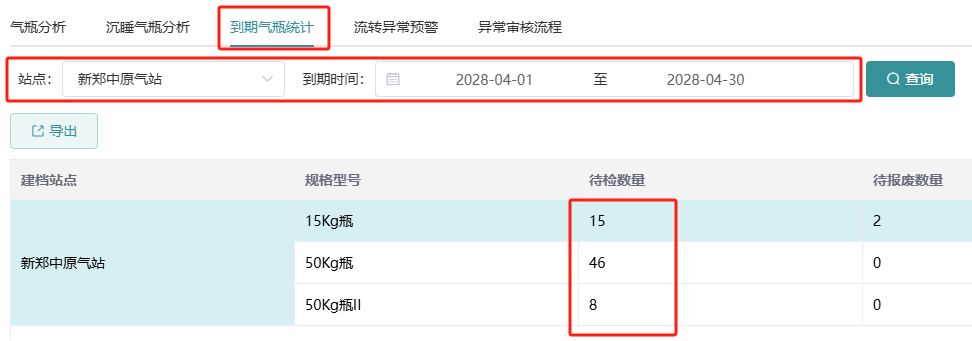
\includegraphics[width=1\textwidth]{dlh_tutorial_figs/overdue}
		\caption{到期气瓶统计}
		\label{fig:overdue}
	\end{figure}
	
	\item 流转异常预警。流转异常类型可以在查询项的“异常类型”中点开查看,由于这里异常类型较多,且与通用设置中的整个流转过程节点关系不大,所以平时没有使用过这个模块。
	
	\item 异常审核流程。这个功能关联设置中的设置--场站配置--流程配置--通用配置 中自定义设置的流程校验以及校验方式,若未开启异常审核流程,则当前这个界面所有异常的审核状态都是“无需审核”。
	
	可以用来检查每天每个库房有哪些配送员未按规范扫码,需要点开芯片编码的链接查看历次流转,必要时需截图保留详细情况,或根据用户联系电话查到造成异常的订单,发给库房核查。
	
	
\end{enumerate}




\subsection{员工管理}

管理气站员工账号信息,可新增,停用、启用、编辑、重置密码。与组织--账号管理不同的是,这里只能管理归属部门为“新郑中原燃气”或“新郑中原气站”的员工账号,不是全局信息,方便赋予对应权限。

\subsection{开票充装}

\textcolor{red}{点击之后弹出新窗口,提示无法访问,新窗口链接是szcz.zzgyjt.cn。}不过公司也没有使用这个功能。

\section{库存}



\subsection{门店库存}
	\begin{itemize}
	
	\item 门店库存。\textcolor{red}{史诗级深坑},总之这里先把一目了然的部分总结一下。可以选择对应门店,勾选“过滤删除的商品”、“过滤下架的商品”,查询对应门店的库存。注意这里的仓库选项默认不为空,只能分库房查看库存。
$$	
\begin{cases}
	\text{期初为上次结转时间当天0点的库存总数量;} \\
	
	\text{入库 = 调入门店+ 配送员还回门店 } \\
	
	\text{出库 = 调出门店+ 配送员领出门店  } \\
	
	\text{盈亏数(盘点模块) = 实际数量 - 账面数量  } \\
	
	\text{盘点模块中的账面数量 = 门店库存页面上次统计的当前库存量} \\
	
	\text{盘盈为正,盘亏为负数。盈亏数为当天所有已提交盘点的所有盈亏数的总和。  } \\
	
	\text{当前库存量 = 期初 + 入库 - 出库 + 盈亏数  } 	
\end{cases}
$$
	
	如果希望当前库存量与实际数量一致,可以尝试根据以上的计算逻辑进行出入库或者盘盈盘亏的加减法,使当前库存量的计算结果等于实际数量。
	
	或者干脆通过“盘点”或“出入库”在前一天下班前把所有库存的当前库存量结果算为0,第二天查看期初数据是否为0,再通过盘点或入库操作,以及前一日下班后配送员的领还单确认数据,将当前库存量的计算结果保持与实际数量一致。\textcolor{red}{总之在保证数量一致前可以通过只填写数量提交单据测试库存结果。数据准确有效后再对后续的出入库气瓶进行扫码和数据提交即可。}
	
	\textcolor{red}{\textbf{但是当我把公式计算通的时候发现,盘点中输入的实际数量又能直接影响当前库存量了,也就是:当前库存量 = 实际数量,上午和下午的几次尝试与结果都不相同,我不懂但是大受震撼。}}如果有相关需求,或需执行调拨管理,可以由管理员使用测试门店多尝试新增几次调拨单或门店盘点,可以暂时不扫码直接提交,发现情况稳定后再推广。
	
	
	\item 出入库查询
	
	门店手动出入库的查询和新增,不走装卸车或领还瓶,只有网页端有这个功能,而且因为是网页端的原因,只能选商品包装物的数量,不能扫码。为了防止被随意使用,因此给所有营业员都关闭了该权限。
	
	\item 库存盘点
	
	可查看门店盘点的所有盘点单
	
	
	
\end{itemize}


\subsection{调拨管理}




\subsection{装卸车单}




\subsection{配送领还单}




\subsection{出入库台账}





\section{商品}

\section{营销}

\section{统计}

\section{组织}

见《河南中原燃气有限公司瓶装燃气平台项目-功能说明文档》4.12.10。

\subsection{组织架构}

见《河南中原燃气有限公司瓶装燃气平台项目-功能说明文档》4.12.10.1。

\subsection{角色权限}

见《河南中原燃气有限公司瓶装燃气平台项目-功能说明文档》4.12.10.2。

作为后台管理员一定要点开每一个角色查看具体权限的勾选情况,以便给某一种角色随时新增或去掉某些功能,或根据具体权限新增某一种角色赋给特定人员。当前角色权限是根据公司具体管理要求设置,没有特别要求一般不能更改。

\subsection{账号管理}

见《河南中原燃气有限公司瓶装燃气平台项目-功能说明文档》4.12.10.3。



\section{设置}
作为网页的管理员,设置中的所有功能和页面都需要尽量熟悉,一些初始的配置和后续更新的功能,都可以在这个部分进行配置。该部分说明请结合实际网页功能查看。

\subsection{配送设置}

\begin{enumerate}
\item 订单分发规则

-预约派单时间,默认开启立即派单。关闭后可以设置预约单的派单时间。但如果手动派单的话应该是不受影响的,猜测是自动派单开启后,这里作为一个关联功能使用。

- 手动派单默认开启不能关闭,默认选中“上次处理人”,这个是手动派单时,派单界面自动填充上一个配送员,如无需修改即可一键派单。

- 自主抢单,这个有点像外卖和网约车的方式,利用手机GPS定位与订单位置,可设置位置区间自动派给订单区域内的配送员;并且可设置接单时间,超时自动再次分配。由于新郑公司给每位配送员定区域定责,因此未使用此功能。

- 自动派单,开启后可设置自动派单规则(注意只是设置规则,要自动派单功能生效需要在下面那一项设置),一般将规则设置为“上次处理人”,可取消勾选“配送员状态必须为‘接单中’”这一项,可以保证所有在职配送员都能接到相应的订单。

- 自主配送单及工单分派方式设置,可以自主选择,在定户定责未完全落实的情况下需要保持手动派单;所有库房均已稳定配送用户后方可开启自动派单,减少派单任务量。把这一项设置为自动派单后,自动派单才会按照上面设置的规则开始生效。

\item 配送附加工单

空的

\item 运费设置

可新增运费设置,根据不同楼层,选择递增或固定金额,无需运费的可将固定金额设为0。在运费设置中设置的顶楼楼层不会影响开户时可选的最高楼层。

\item 配送配置

- 随配送单关联安检,开启后在完成订单的“随单任务”里显示必做,完成后方可进入订单下一步操作。

- 随配送单合同签署,验证对应用户户号的用户是否已签署供气协议,即后续合同配置中上传的合同模板。若该户号的用户未签署过合同,则“随单任务”中会有这一项,若已签署合同,则不会出现该任务。

- 随配送单验证开户必填信息,字面意思。开户时一般会要求将必填信息填写后才完成开户。但开户必填信息是可以在系统上配置的,如果开户时有些信息非必填但是后续设置了必填,那这个功能开启时会验证并要求填写。

- 运气到家开启离线签单,这个功能网页中有详细解释,由于该功能开启后无法进行安检等必做任务,因此新郑公司未使用。

- 随配送单更新用户就近门店与订单门店,非常重要的功能,如果你需要统计用户数据,需要区分各库房任务,需要各库房营业员为老客户精准派单,这个功能可谓神来一笔,能解决大部分的问题,无脑开。

\end{enumerate}


\subsection{销售设置}
\begin{enumerate}
	\item 销售渠道设置
	
	保存了一些渠道名称和对应ID,可新增。平时用不到这个模块。
\end{enumerate}


\subsection{财务设置}

这一部分需要根据财务的具体要求设置,如果有任何切换需求,要先跟多立恒确认具体方法,或者由多立恒的陈腾经理直接处理。

\begin{enumerate}
	\item 支付方式设置
	
	\begin{itemize}
		 
	\item 可按需将列举的支付方式更名、启用或停用。在对应的支付方式--编辑中,可配置相应的接口信息。

	\end{itemize}

	\item 支付渠道设置
	\begin{itemize}
		
		\item 微信商城支付配置,用户在微信上下单的各项付费业务的支付方式权限,可按不同部门配置权限。“微信商品下单启用货到付款”即不限制微信下单必须付款后再生成订单,权限按门店配置。
		
		\item 运气到家支付配置,送气工在app上代客下单时的各项付费业务的支付权限,可按不同部门配置权限。
		
		\item 平台支付配置,网页端客服或营业员下单时的支付配置。
		
	\end{itemize}



\end{enumerate}


\subsection{微信配置}
\begin{enumerate}
	\item 一键订气配置
	
	配置“微信订气”首页的界面组件。可在中间界面图片中点击对应位置的组件,并在右侧显示的组件详情中自行配置。其中,左侧的组件库也可拖拽至中间界面图片想要的位置中,自行配置页面布局。
	
	\item 个人中心配置
	
	配置“微信订气”中“个人中心”的功能模块。可自行配置所需显示给用户的功能,以及显示位置。但是“发票”功能是2024.12月的新功能,新郑公司未使用,因此未对使用方式进行了解。
	
	\item 公众号配置
	
	公司申请服务号后由多立恒配置新增。
	
	\item 微信业务配置
	
	配置微信订单的待支付时限;配置微信端配送中是否显示配送员详细信息,姓名、电话号码等。
\end{enumerate}


\subsection{工单配置}
\begin{enumerate}
	\item 工单配置
	在好运气app首页的“工单”中列出的工单选项。
	报修、
	投诉、
	咨询。
	可按需新增,新郑公司在该模块中新增了“沉睡气瓶排查单”工单,用于上传沉睡气瓶告知书,保存相应的用户信息与告知书下发原因。
	
	\item 附加工单配置
	
	附加工单配置可自行新增,附加工单启用是也是在在好运气app首页的“工单”中显示。
	
	
\end{enumerate}



\subsection{安检配置}
\begin{enumerate}
	\item 安检模板配置
	
	\begin{itemize}
		

	\item \textcolor{red}{定期安检和随单安检有区分}
	
	首次安检均为定期安检,并且超出设置的安检周期的次回安检会自动归类为定期安检(已查到间隔三天的两次安检一次是随单,最新一次是定期;但是系统判断该用户的上次安检时间是三个月前(之前设置的定期安检周期)的某一次,而只有这两次被归类为定期安检。期间的其他多次安检都是随单安检类型)。验证方法:将定期安检周期增加为一年一次(新郑目前没有超过一年的安检单),次日的所有安检单中只有新用户的安检单被分类为定期安检,其余全部是随单安检。验证结果:√。PS:20250407更新,新的定期安检也有老用户,而且不是一年以上的安检。PS:20250415更新,多立恒确认了这个定期安检的认定方法,那几个特殊情况就当不存在吧。
	
	
	\item 安检模板配置--编辑:可设置安检单名称,选择适用用户类型,适用用户门店,以及安检周期。如果不同门店或不同类型用户的安检内容不一样,可以复制新增多个安检模板,并在对应模板内修改。安检周期设置后,如果用户上次安检时间超过了设置的时间,用户在微信订气的“个人中心”中会显示“安检已超期”字样,网页上用户安检的信息中也会有同样提示。可根据公司的管理制度决定是否需要配送员上门进行定期安检。
	
    \item 安检模板配置--安检项配置:可根据地区的相关法律法规新增安检项,可为安检项的每个条目设置隐患等级,如需整改,可自定义整改意见。隐患等级以及是否需要整改可在“隐患配置”中配置。
	
	\end{itemize}
	
	\item 隐患配置
	\begin{itemize}
		\item 
	
	可新增或设置隐患名称,是否需整改,以及状态是否启用。用于安检模板中的安检项隐患选项。
	\end{itemize}
	\item 其他配置
	
	\begin{itemize} 
	
	\item 位置异常标记,可设置安检位置超出用户地址的距离,设置并保存后,安检单管理中“位置偏差”一列会显示实际超出的距离。未超出的不显示。
	
	\item 定期安检审核,随单安检审核。这两个功能开启后在“安检单管理”中,每条安检信息后会有“审核”功能,需要在网页中手动审核,方可在流程中完成整个安检。开启审核后,未经审核的安检单仍可以修改安检中的勾选选项以及上传照片。
	
	\item 整改审核,有隐患的安检单会在配送员的好运气app上保留一个整改任务,若通过这个整改入口重新整改勾选安检项,提交后仍需“审核”。
	
	\item 随单安检更新用户上次安检时间,“用户管理”页面中的用户信息有一个“上次安检时间”,如果这个配置开启,那么手动审核后才会在这一列更新上次安检时间,否则不会更新。
	
	\item 安检后立即更新用户安检时间,这个功能开启后无需依赖手动审核,安检时间直接根据安检的提交时间上传更新在用户管理中的“上次安检时间”位置。
	\end{itemize}

\end{enumerate}


\subsection{用户配置}
\begin{enumerate}
	\item 开户设置
	
	设置开户信息模板,可编辑。开户设置已有的控件都是系统内置无法修改的,也就是说开户时楼层选择是根据法律法规要求的1-9层,不能根据公司的管理规定修改成更低楼层。
	
	\item 用户类型
	
	用户类型可新增,可编辑。该模块会影响所有用户类型相关查询,商品或安检的适用用户类型等。
	
	\item 开户配置
	
	开户配置:开户后自动创建工单,有需要的可以用。实名开户配置,这个配置主要是实名认证需求,比如工业用户,按公司管理要求可开启企业或个人的信息认证。开启后,用户选择工业类型,则个人或企业信息会成为必填项,用户需填写后方可成功开户。
	
	开户须知:开户须知可自行编辑填写。
	
	\item 用户标签
	
	可自行配置,一般无特殊需求可以不设置。
	
	\item 合同模板管理
	
	见《河南中原燃气有限公司瓶装燃气平台项目-功能说明文档》4.3.3.2。
	
\end{enumerate}

\subsection{溯源配置}
\begin{enumerate}
	
	\item 一户一码配置
	
	这个功能配置的是每个用户户号对应的唯一二维码扫码时展示的页面。
	
	\begin{itemize}
		\item 组件库,可将相应的组件名称拖拽至UI界面的相应位置,自定义搭配。
		\item 轮播图片,界面最上端图片最多可轮播6张图片,建议长宽比3:1。
		\item 用户信息,可自定义该界面展示的用户信息,包含用户基础信息以及部分用气信息。
		\item 在用气瓶信息,展示现场配送节点在对应用户处的气瓶,包含气瓶编号与芯片编码。
		\item 用气统计,可按时间区间展示最多近1年的订气瓶数。
		\item 配送信息,可选择展示最近x次配送,可选显示字段“配送时间”,“配送车辆”,“配送员”。
		\item 安检信息,可选择展示最近x次安检。该模块在实际界面中可点击“详情”查看详细安检情况。
		\item 订气渠道入口,可勾选两种渠道,“电话订气”、“微信订气”。
	\end{itemize}
	
	\item 一瓶一码配置
	
	这个功能配置的是瓶身安装的已建档的芯片二维码扫码时展示的页面。
	
	\begin{itemize}
		\item 组件库,可将相应的组件名称拖拽至UI界面的相应位置,自定义搭配。
		\item 页面标题,标题可自定义。
		\item 轮播图片,轮播图片,界面最上端图片最多可轮播6张图片,建议长宽比3:1。
		\item 使用预警,用户气瓶超时未流转不合格预警设置。可自定义搭配用户类型、气瓶类型、超时天数设置预警信息,可新增多个预警条件。相应用户类型、气瓶类型超期的气瓶,扫描瓶身二维码时会显示使用预警信息以及显眼的“疑不明气源”红码标识。
		\item 气瓶信息,可勾选列举的所有气瓶信息,该信息详情与网页内气瓶建档导入的信息关联,与气瓶厂家出厂信息不直接相关。
		\item 流转信息,所有流转信息可勾选展示,可公司实际管理要求勾选具体的展示类别和每个类别内展示的具体项目。这个信息的详细内容因为是一个气瓶完整的追溯项目,所以建议完整查看一遍。
	\end{itemize}
	
	
	\item 一车一码配置
	
	这个功能配置的是网页中 配送--车辆管理 中,新增车辆生成的唯一二维码扫码时的展示页面。
	\begin{itemize}
		\item 组件库,可将相应的组件名称拖拽至UI界面的相应位置,自定义搭配。
		\item 车辆信息,此信息与 配送--车辆管理 中的录入信息关联,可自定义配置可扫码获得的数据项。
		\item 员工信息,此信息包含“司机”与“押运员”,车辆管理-新增车辆 时,需从系统账号管理已有的人员中选择人员作为司机和押运员,人员对应信息与账号管理中写入的信息关联。可自定义配置扫码获得的数据项。
		\item 库存详情,可展示该车辆中存放的重瓶、空瓶,及其对应的规格、数量、气瓶号、芯片编码。该信息与气瓶流转信息关联,若流转扫码节点最终位置在车辆对应的配送员或司机处时,气瓶信息将会更新至车辆的库存信息中。
		\item 配送信息,与气瓶流转信息关联,车辆对应的配送员送出扫码时更新此项目数据。
		\item 预警信息,目前不清楚使用场景与关联更新模块。
	\end{itemize}
	
	
\end{enumerate}


\subsection{场站配置}

\begin{enumerate}
	\item 场站字典
	
	\item 建档配置
	
	\item 充装检查
	
	\item 充装排班
	
	\item 流程配置
	
		\begin{itemize}
			
		\item 流程配置
		
		点开每一个流程节点查看可设置的验证功能,可以选择“开启”、“关闭”列出的验证项,也可以“新增”验证项。\textcolor{red}{但是“配送回收”节点只能验证扫码数量等一些常规项,不能验证气瓶回收的用户是否为“现场配送”时对应的用户。}
		
		\item 通用配置
		
		- 流程审核设置,可以勾选流程校验、设置校验时是否跳过,以及校验异常时的处理方法“异常拦截”、“异常提醒”、“流程异常审核”。出现异常流程后会显示在“气站”--“气瓶分析”--“异常审核流程”中。
		
		- 如果设置勾选了“流程异常审核”,就需要在审核流程页面中手动审核;如果需要日常排查流转异常节点以及异常处理人,可以直接在“气站”--“气瓶分析”--“异常审核流程”页面中筛选查询条件依次查看异常信息。
		
		- 目前该设置无需更改,但是如果管理方法能规定下来营业员必须在配送员领还瓶时即时确认领还单(如果管理人员能去每个现场盯着这项工作执行一段时间或许可以有效),那么就可以把“配送领瓶”、“配送还瓶”的“跳过”勾选取消,将领还瓶也作为一项卡死的流程校验,甚至可以在部分流程中设置“流程异常审核”要求营业员手动审核异常流程,避免配送员胡乱扫码做虚假订单。
		
		\item 调拨配置
		
		配置危运车在气站、库房之间的调拨设置,由于新郑公司完全未启用调拨管理,因此未做更改。之前给营业员的调拨扫码简化版流程其实是可以用的,如果能多测试几次就可以找到正确使用方法,或者可以在一周内根据前一天库存数量将正确的气瓶库存数和扫码气瓶对应下来。但是财务和营业员发现一次异常后没有再继续配合调拨的扫码测试,这也是流程无法全面把关的漏洞之一。或许跟上面一样管理人员去每一个库房现场盯一段时间会有用。
		

		\end{itemize}
	
	\item 气瓶标签
	
	\item 一码到底
	
	
	
\end{enumerate}


\subsection{营销配置}

\begin{enumerate}
	\item 积分规则配置
	
	\item 会员等级规则配置
	
\end{enumerate}


\subsection{消息配置}

\begin{enumerate}
	\item 消息配置
	
	\item 消息记录
	
	\item 渠道配置
	
\end{enumerate}


\subsection{呼叫中心配置}

\begin{enumerate}
	\item 呼叫中心管理
	
	可以查看呼叫中心号码,绑定话务员,查看坐席状态,以及呼叫中心到期时间,这个到期时间是什么建议问一下多立恒,不然到期后造成客服电话无法使用还需要再次处理。
	
	\item 上班时间配置
	
	与“下班转接配置”配合使用,“起始结束月份”和“起始结束日期”是按照阳历年设置,如果需要跳过春节假期,则应该分段录入起始时间,假期期间的“起始结束时间”部分可以设置为“00:00--00:01”之类的。具体情况过年的时候多立恒会指导。2024-2025年度的设置已删除,避免影响2025-2026年度的时间安排。
	
	\item 下班转接配置
	
	下班转接指的是上文中设置的“上班时间”以外的时间,可根据门店和日期期间根据各库房上报的值班信息按照每天、每人、每库房依次录入,会比较花时间,需要耐心。如果转接人信息长度超出页面且没有滚动轮下滑的话,可以缩小页面显示比例调整一下,再进行新增。
	
	\item 黑名单管理
	
	录入不再接听的电话号码后系统会屏蔽对应的电话号码。
	
	\item 话务员管理
	
	\item 区域坐席配置
	
\end{enumerate}


\subsection{其他配置}

\begin{enumerate}
	\item 公司信息
	
	\item 电脑打印模板
	
	\item 手机打印模板
	
	\item 操作日志
	
	这个功能很有用,你可以在这里查到所有气瓶档案中被标记无效的原气瓶编号。所有可查看操作的模块可在“模块”查询框中选择。慎重更改系统中的信息,因为会在这里被记录。
	
	\item 登录日志
	
	这个功能也很有用,如果有的配送员账号总是莫名其妙被停用,有可能是其他配送员把账号记错,误登他的号,但是不知道密码,所以多次尝试后被停号了。这个时候就可以查一下他的账号都被什么型号的手机或者哪个登录IP尝试登录了。如果你有耐心,可以顺藤摸瓜翻一下近几天的所有登录日志,找到另一个一样的手机型号对应的账号,即可查到登号的那个人,一般两个账号相似度比较高,查的时候很容易看出来。
	
	\item 三方接入
	
	\item 字典配置
	
\end{enumerate}


\end{document}














